\section{Coverage Audit and Inferential Informativeness}
\setcounter{equation}{0}\setcounter{table}{0}\setcounter{figure}{0}
\label{app:coverage-forensic-audit}

\subsection{Direct-at-Truth Coverage Audit}

Coverage is evaluated directly at the exact true structural effect $\alpha_0(\tau)$, independently of whether that value lies on the finite candidate grid. The forensic audit checked 60,000 direct truth evaluations: 500 replications for each of 120 sample-size, quantile, instrument-strength, and estimator cells.

Wilson 95\% Monte Carlo intervals exclude nominal $0.95$ coverage in 54 of the 120 cells. The audit finds no missing or nonfinite true-parameter $W$ statistics. The large coverage distortions reported in the main text are therefore neither plotting-grid artifacts nor consequences of missing-value handling. The frozen audit report and supporting diagnostics remain preserved in the repository. Wilson intervals are pointwise Monte Carlo uncertainty intervals, without simultaneous or multiplicity-adjusted significance claims. An individual rate's Monte Carlo standard error is not a standard error for a difference between correlated simulation results.

These checks rule out those numerical explanations for the reported coverage patterns. They do not establish correct theoretical specification, validate the asymptotic reference distribution for this DGP, or establish nominal finite-sample calibration.

\subsection{Coverage-Audit Summary}

Table~\ref{tab:coverage-audit-summary} summarizes the audit by estimator and sample size. Each row contains 20 quantile--$\kappa$ cells. Recalculation from integer acceptance counts reproduces 53 cells with an upper Wilson endpoint below 0.95 and one with a lower endpoint above 0.95, giving the reported total of 54. Comparisons use unrounded endpoints and the same 500-evaluation denominator in every cell.

\begin{table}[!ht]
\caption{Direct-at-truth coverage audit.}
\label{tab:coverage-audit-summary}
\centering
\begin{tabular}{lrrrrrrr}
\toprule
Estimator & $n$ & Cells & \shortstack{Coverage\\min.} & \shortstack{Coverage\\max.} & \shortstack{Upper\\$<0.95$} & \shortstack{Lower\\$>0.95$} & \shortstack{Missing/\\nonfinite} \\
\midrule
Oracle-GMM & 500 & 20 & 0.858 & 0.954 & 6 & 0 & 0 \\
Oracle-GMM & 1000 & 20 & 0.860 & 0.964 & 8 & 0 & 0 \\
Full-GMM & 500 & 20 & 0.442 & 0.962 & 9 & 0 & 0 \\
Full-GMM & 1000 & 20 & 0.502 & 0.962 & 12 & 0 & 0 \\
DML-IVQR & 500 & 20 & 0.658 & 0.976 & 8 & 1 & 0 \\
DML-IVQR & 1000 & 20 & 0.498 & 0.968 & 10 & 0 & 0 \\
\bottomrule
\end{tabular}
\begin{tablenotes}
Each row covers 20 quantile--$\kappa$ cells, with 500 direct-at-truth evaluations per cell. Coverage is reported as a proportion. The upper/lower columns count cells whose unrounded Wilson upper endpoint is below 0.95 or lower endpoint is above 0.95. Intervals use integer acceptance counts, the verified denominator, and the two-sided 95\% Wilson formula without continuity correction. They are pointwise Monte Carlo intervals, not simultaneous or multiple-testing-adjusted intervals; exclusion counts are descriptive audit summaries. Missing/nonfinite counts concern direct-at-truth $W$ evaluations (missing values are counted once).
\end{tablenotes}
\end{table}

\FloatBarrier

\subsection{Full-Domain Grid Acceptance}

The domain-expansion diagnostics in Appendix~\ref{app:numerical-domain-diagnostics} are complemented by Figure~\ref{fig:appendix_full_domain_acceptance}, which reports how often every evaluated point in the primary domain is accepted. Reading this frequency alongside coverage distinguishes retention of the true effect from the ability to exclude competing candidates within the maintained domain. Coverage near nominal can coexist with frequent acceptance of all primary-grid candidates: retaining the true value does not imply excluding alternatives.

The heatmap uses stored grid-profile evaluations, whereas coverage uses a separate evaluation directly at truth. These are distinct computations; in DML-IVQR, fresh pivotal draws can differ between them, so their acceptance events need not coincide even when truth is a grid point. Full-domain grid acceptance refers only to the 41 evaluated points in $A_0=[-1,3]$, not to acceptance of the real line or global unboundedness of an unrestricted confidence region.

\begin{figure}[!ht]
  \centering
  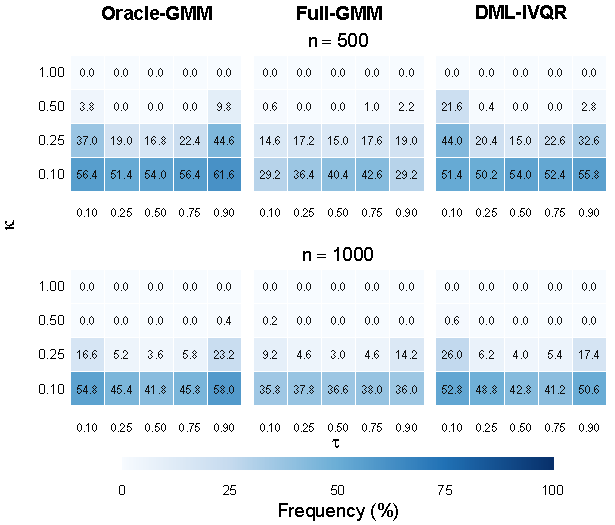
\includegraphics[width=0.72\textwidth]{figures/generated/full_domain_acceptance_heatmap.pdf}
  \caption{Full-domain grid acceptance frequencies.}
  \label{fig:appendix_full_domain_acceptance}
  \begin{figurenotes}
    Each cell reports the percentage of 500 complete replications accepting all 41 evaluated grid points in $A_0=[-1,3]$, with step size $h=0.1$. Panel columns identify estimators; panel rows show $n=500$ and $n=1000$. Within each panel, columns show quantiles $\tau$ and rows show relevance $\kappa$, declining from 1.00 to 0.10. Darker shading on the shared 0--100\% scale means more frequent full-domain grid acceptance. This event neither denotes acceptance of the entire real line nor establishes an unbounded unrestricted confidence region.
  \end{figurenotes}
\end{figure}

\FloatBarrier
